%%%%%%%%%%%%%%%%%%%%%%%%%%%%%%%%%%%%%%%%%
% Article EcoFoG
% Version 2.1 (23/10/2017)
%
% adapté de :
% Stylish Article
% LaTeX Template
% Version 1.0 (31/1/13)
%
% This template has been downloaded from:
% http://www.LaTeXTemplates.com
%
% Original author:
% Mathias Legrand (legrand.mathias@gmail.com)
%
% License:
% CC BY-NC-SA 3.0 (http://creativecommons.org/licenses/by-nc-sa/3.0/)
%
%%%%%%%%%%%%%%%%%%%%%%%%%%%%%%%%%%%%%%%%%


%----------------------------------------------------------------------------------------
%	PACKAGES AND OTHER DOCUMENT CONFIGURATIONS
%----------------------------------------------------------------------------------------

\documentclass[fleqn,10pt]{ArtEcoFoG} % Document font size and equations flushed left

\setcounter{tocdepth}{3} % Show only three levels in the table of contents section: sections, subsections and subsubsections


% Pandoc environments
\usepackage{framed}
\usepackage{fancyvrb}
\providecommand{\tightlist}{%
  \setlength{\itemsep}{0pt}\setlength{\parskip}{0pt}}
\newcommand{\VerbBar}{|}
\newcommand{\VERB}{\Verb[commandchars=\\\{\}]}
\DefineVerbatimEnvironment{Highlighting}{Verbatim}{commandchars=\\\{\}, fontsize=\scriptsize} % Code R
\definecolor{shadecolor}{RGB}{248,248,248}
\newenvironment{Shaded}{\begin{snugshade}}{\end{snugshade}}
\newcommand{\KeywordTok}[1]{\textcolor[rgb]{0.13,0.29,0.53}{\textbf{{#1}}}}
\newcommand{\DataTypeTok}[1]{\textcolor[rgb]{0.13,0.29,0.53}{{#1}}}
\newcommand{\DecValTok}[1]{\textcolor[rgb]{0.00,0.00,0.81}{{#1}}}
\newcommand{\BaseNTok}[1]{\textcolor[rgb]{0.00,0.00,0.81}{{#1}}}
\newcommand{\FloatTok}[1]{\textcolor[rgb]{0.00,0.00,0.81}{{#1}}}
\newcommand{\ConstantTok}[1]{\textcolor[rgb]{0.00,0.00,0.00}{{#1}}}
\newcommand{\CharTok}[1]{\textcolor[rgb]{0.31,0.60,0.02}{{#1}}}
\newcommand{\SpecialCharTok}[1]{\textcolor[rgb]{0.00,0.00,0.00}{{#1}}}
\newcommand{\StringTok}[1]{\textcolor[rgb]{0.31,0.60,0.02}{{#1}}}
\newcommand{\VerbatimStringTok}[1]{\textcolor[rgb]{0.31,0.60,0.02}{{#1}}}
\newcommand{\SpecialStringTok}[1]{\textcolor[rgb]{0.31,0.60,0.02}{{#1}}}
\newcommand{\ImportTok}[1]{{#1}}
\newcommand{\CommentTok}[1]{\textcolor[rgb]{0.56,0.35,0.01}{\textit{{#1}}}}
\newcommand{\DocumentationTok}[1]{\textcolor[rgb]{0.56,0.35,0.01}{\textbf{\textit{{#1}}}}}
\newcommand{\AnnotationTok}[1]{\textcolor[rgb]{0.56,0.35,0.01}{\textbf{\textit{{#1}}}}}
\newcommand{\CommentVarTok}[1]{\textcolor[rgb]{0.56,0.35,0.01}{\textbf{\textit{{#1}}}}}
\newcommand{\OtherTok}[1]{\textcolor[rgb]{0.56,0.35,0.01}{{#1}}}
\newcommand{\FunctionTok}[1]{\textcolor[rgb]{0.00,0.00,0.00}{{#1}}}
\newcommand{\VariableTok}[1]{\textcolor[rgb]{0.00,0.00,0.00}{{#1}}}
\newcommand{\ControlFlowTok}[1]{\textcolor[rgb]{0.13,0.29,0.53}{\textbf{{#1}}}}
\newcommand{\OperatorTok}[1]{\textcolor[rgb]{0.81,0.36,0.00}{\textbf{{#1}}}}
\newcommand{\BuiltInTok}[1]{{#1}}
\newcommand{\ExtensionTok}[1]{{#1}}
\newcommand{\PreprocessorTok}[1]{\textcolor[rgb]{0.56,0.35,0.01}{\textit{{#1}}}}
\newcommand{\AttributeTok}[1]{\textcolor[rgb]{0.77,0.63,0.00}{{#1}}}
\newcommand{\RegionMarkerTok}[1]{{#1}}
\newcommand{\InformationTok}[1]{\textcolor[rgb]{0.56,0.35,0.01}{\textbf{\textit{{#1}}}}}
\newcommand{\WarningTok}[1]{\textcolor[rgb]{0.56,0.35,0.01}{\textbf{\textit{{#1}}}}}
\newcommand{\AlertTok}[1]{\textcolor[rgb]{0.94,0.16,0.16}{{#1}}}
\newcommand{\ErrorTok}[1]{\textcolor[rgb]{0.64,0.00,0.00}{\textbf{{#1}}}}
\newcommand{\NormalTok}[1]{{#1}}
\usepackage{longtable,booktabs}
\usepackage{caption}
% These lines are needed to make table captions work with longtable:
\makeatletter
\def\fnum@table{\tablename~\thetable}
\makeatother
% longtable 2 columns
% https://tex.stackexchange.com/questions/161431/how-to-solve-longtable-is-not-in-1-column-mode-error
\makeatletter
\let\oldlt\longtable
\let\endoldlt\endlongtable
\def\longtable{\@ifnextchar[\longtable@i \longtable@ii}
\def\longtable@i[#1]{\begin{figure}[t]
\onecolumn
\begin{minipage}{0.5\textwidth}\scriptsize
\oldlt[#1]
}
\def\longtable@ii{\begin{figure}[t]
\onecolumn
\begin{minipage}{0.5\textwidth}\scriptsize
\oldlt
}
\def\endlongtable{\endoldlt
\end{minipage}
\twocolumn
\end{figure}}
\makeatother

\usepackage{graphicx,grffile}
\makeatletter
\def\maxwidth{\ifdim\Gin@nat@width>\linewidth\linewidth\else\Gin@nat@width\fi}
\def\maxheight{\ifdim\Gin@nat@height>\textheight0.8\textheight\else\Gin@nat@height\fi}
\makeatother
% Scale images if necessary, so that they will not overflow the page
% margins by default, and it is still possible to overwrite the defaults
% using explicit options in \includegraphics[width, height, ...]{}
\setkeys{Gin}{width=\maxwidth,height=\maxheight,keepaspectratio}

% User-adder preamble
\usepackage{textcomp} \DeclareUnicodeCharacter{B0}{\textdegree}
\usepackage{tabu}
\renewenvironment{table}{\begin{table*}}{\end{table*}\ignorespacesafterend}
\hyphenation{bio-di-ver-si-ty sap-lings post-dis-tur-bance}
\hypersetup{draft}

%----------------------------------------------------------------------------------------
%	ARTICLE INFORMATION
%----------------------------------------------------------------------------------------

\JournalInfo{\ }
\Archive{\ }

\PaperTitle{30 Years of Post-disturbance Recruitment in a Neotropical Forest} % Article title

\Authors{
Ariane MIRABEL\textsuperscript{1*}\\ Eric MARCON\textsuperscript{1}\\ Bruno HERAULT\textsuperscript{2}
} % Authors
\affiliation{
\textsuperscript{1}UMR EcoFoG, AgroParistech, CNRS, Cirad, INRA, Université des Antilles,
Université de Guyane.\\ \hspace{1em} Campus Agronomique, 97310 Kourou, France.\\\textsuperscript{2}INPHB (Institut National Polytechnique Félix Houphoüet Boigny)\\ \hspace{1em} Yamoussoukro, Ivory Coast
}
\affiliation{*\textbf{Corresponding author}: ariane.mirabel@ecofog.gf, https://github.com/ArianeMirabel} % Corresponding author

\Keywords{Disturbance Dynamics, Neotropical Forests, Recruitment, Resilience, Taxonomic and Functional Diversity, Tree Community} % Keywords - if you don't want any simply remove all the text between the curly brackets
\newcommand{\keywordname}{Keywords} % Defines the keywords heading name

%----------------------------------------------------------------------------------------
%	ABSTRACT
%----------------------------------------------------------------------------------------

\Abstract{
The role of tree diversity for tropical forests functioning and services
makes it crucial tree diversity and composition fate in the global
changing context. Community long-term response to disturbance rely on
tree recruitment, long seen as following deterministic successional
pathways. These pathways however might be altered in the hyper-diverse
tropical forests and of slight but recurrent disturbances induced by
global changes. Post-disturbance recruitment trajectories would (i)
disentangle the determinants of tree recruitment between stochastic and
deterministic processes that enhance a restricted pool of species, and
(ii) elucidate tropical forests taxonomic and functional resilience. We
examined the trajectories over 30 years of recruited trees taxonomic and
functional diversity in 75 ha of forest following a disturbance
gradient. We analyzed taxonomic richness, evenness, and turnover, and
functional diversity and composition (regarding 7 leaf, stem and
life-history functional traits). We highlighted a three-phased
successional pathway defined by the interplay of stochastic and
deterministic recruitment processes. The succession translated into (i)
saplings growth mirroring pre-disturbance communities, (ii)
light-demanding species enhanced recruitment entailing, above a
disturbance intensity threshold, the dominance of pioneers and (iii) the
recovery of pre-disturbance taxonomic and functional characteristics and
of stochastic recruitment processes. Although tangible, community
taxonomic and functional resilience was decades-long. Post-disturbance
recruitment relied on deterministic competition processes for light
balancing the stochastic processes ruling undisturbed communities.
Although resilient, recruitment taxonomic and functional characteristics
remained altered in the long-term, calling caution for forest
management.
}

%----------------------------------------------------------------------------------------

\begin{document}

\selectlanguage{english}

\flushbottom % Makes all text pages the same height

\maketitle % Print the title and abstract box

\tableofcontents % Print the contents section

\thispagestyle{empty} % Removes page numbering from the first page

%----------------------------------------------------------------------------------------
%	ARTICLE CONTENTS
%----------------------------------------------------------------------------------------








\section{Introduction}\label{introduction}

Determining the response of tropical forests to disturbance is key to
predict their fate in the global changing context. In the last decades,
tropical forests experienced a wide range of disturbance, from radical
land-use changes for agriculture or mining
\citep{Dezecache2017a, Dezecache2017b} to more insidious changes
following climatic changes or anthropogenic activities like selective
logging \citep{Baraloto2012a, Aubry-Kientz2015}. In that respect a vast
literature successfully modeled community response to disturbance in
terms of tree growth, tree height and fluxes of carbon, water and
nutrients
\citep{Gourlet-Fleury2000, Putz2012, Piponiot2016, Rutishauser2016}.
Regarding tree community diversity and composition, the ecological
theory of succession assumes that disturbance initiates a suit of
deterministic recruitment processes depending on species resource use
and competitive abilities \citep{Clements1916, Meiners2015}. The
successional framework then assumes predictable trajectories driving a
gradual recovery of the pre-disturbance
\citep{Chesson2000, Rees2001, Adler2007}. Specifically in forest
ecosystem, this succession comprises first the recruitment of saplings
benefiting from the available resources and the low competition, then
into the progressive exclusion of low-competitive species following
stand maturation, and eventually the senescence of early-successional
and the emergence of late-successional species restoring the
pre-disturbance state \citep{Denslow2000}. Empirical evidence, however,
show that post-disturbance trajectories often deviate from the predicted
successional pattern and then result from the interplay between
deterministic and stochastic processes. Post-disturbance trajectories
then depend as well on random processes, like dispersal limitations, and
may lead to different equilibrium state
\citep{Hubbell2001, Chave2004, Norden2015}. Specifically for tropical
forests, where the diversity is huge and the long-term monitoring are
scarce, the balance between deterministic and stochastic processes
remains debated. While several studies highlighted predictable and
homogeneous successional patterns towards the resilience of
pre-disturbance state \citep{Norden2009, Letcher2015}, other showed
diverging post-disturbance trajectories and different equilibrium state
\citep{Longworth2014, Norden2015}. The convergence of post-disturbance
trajectories might be missed if some facets of community diversity are
overlooked. The interplay of determinisitic and stochastic processes
might translate into a divergence in the taxonomic space, with the
random recruitment of species, and a converge in the functional space,
with different functional characteristics fostered along the trajectory
\citep{Fukami2005, Li2018}.

Ecological processes affect both community taxonomic characteristics,
that refer to neutral species assemblages, and functional
characteristics, that account for species ecology and functioning
\citep{Macarthur1967, Violle2007b, Kunstler2016}. The different
ecological processes can be assessed through the taxonomic and
functional diversity and composition of recruited communities following
disturbance \citep{Fukami2005, Chalmandrier2015, Cequinel2018}. A
determinisitic succession thus imply predictable recruitment
trajectories comprising a succession of recruitment processes based on
species competitive ability \citep{Rees2001, Perronne2017}. In tropical
forests, light is the limiting resource: post-disturbance trajectories
would be shaped by a shift from slow-growing, long-lived species with
``conservative'' resource use, to fast-growing species with
``acquisitive'' resource use
\citep{Denslow1980, Molino2001, Bongers2009}.\\
Key leaf, wood and life-history functional traits assessing species
resources acquisition strategy and ecology would then grasp the
competition processes at stake
\citep{Wright2004, Chave2009b, Herault2011}. The balance between
deterministic and stochastic processes would translate in a random
divergence of both community trajectories, contrasting with a
deterministic convergence towards the recovery pre-disturbance state
\citep{Clements1916, Diamond1975}.

In this paper we followed recruitment trajectories over 30 years of 75
ha of Neotropical forest plots set up on a gradient of disturbance
intensity, from 10 to 60\% of forest biomass removed. We examined the
recruited trees (i) taxonomic composition, richness and evenness, (ii)
taxonomic turnover compared to pre-disturbance community, and (iii)
functional composition and diversity based on seven major leaf, stem and
life-history traits. We compared the recruitment trajectories to neutral
models corresponding to a stochastic recruitment and a randomization of
species functional traits. Specifically, we (i) elucidated the
successional pathway shaping community response to disturbance and the
underlying ecological processes and (ii) clarified the extent of
community taxonomic and functional resilience,in the sense of
pre-disturbance characteristics recovery, and its consequences for
tropical forest management.

\section{Material and Methods}\label{material-and-methods}

\subsection{Study Site}\label{study-site}

The Paracou station is located in a lowland tropical rainforest in
French Guiana (518\textdegree N and 5253\textdegree W). Climate is
tropical wet with mean annual precipitation averaging 2980
mm.yr\textsuperscript{-1} (30-yr period) and a 3-months dry season
(\textless{} 100 mm.mo\textsuperscript{-1}) from mid-August to
mid-November, and a one-month dry season in March \citep{Wagner2011}.
Elevation ranges from 5 to 50 m and mean annual temperature is
26\textdegree C. Soils are thin acrisols over a layer of transformed
saprolite with low permeability generating lateral drainage during heavy
rains. The experiment is a network of twelve 6.25 ha plots (Table
\ref{tab:Tab1}) that underwent three disturbance treatments in 1987
according to a randomized plot design with three replicate blocks of
four plots \citep{Herault2018}.

\begin{table}

\caption{\label{tab:Tab1}Intervention table, summary of the disturbance intensity for the 4 plot treatments in Paracou.}
\centering
\begin{tabu} to \linewidth {>{\raggedright}X>{\raggedright}X>{\raggedright}X>{\raggedright}X>{\raggedright}X}
\toprule
Treatment & Timber & Thinning & Fuelwood & \%AGB lost\\
\midrule
Control & - & - & - & 0\\
T1 & DBH $\geq$ 50 cm, commercial species, $\approx$ 10   $trees.ha^{-1}$ & - & - & $[12-33]$\\
T2 & DBH $\geq$ 50 cm, commercial species, $\approx$ 10  $trees.ha^{-1}$ & DBH $\geq$ 40 cm, non-valuable species, $\approx$ 30   $trees.ha^{-1}$ & - & $[33-56]$\\
T3 & DBH $\geq$ 50 cm, commercial species, $\approx$ 10  $trees.ha^{-1}$ & DBH $\geq$ 50 cm, non-valuable species, $\approx$ 15  $trees.ha^{-1}$ & 40 cm $\leq$ DBH $\leq$ 50 cm, non-valuable species,\ $\approx$ 15 $trees.ha^{-1}$ & $[35-56]$\\
\bottomrule
\end{tabu}
\end{table}

\subsection{Inventories Protocol and Dataset
Collection}\label{inventories-protocol-and-dataset-collection}

Dominant families in the study site are Fabaceae, Chrysobalanaceae,
Lecythidaceae and Sapotaceae. All trees above 10 cm DBH were mapped and
measured annually since 1984. Trees are first identified with a
vernacular name assigned by the forest worker team, and afterward with a
scientific name assigned by botanists during regular botanical
campaigns. Botanical campaigns have been carried out every five to six
years from 2003 onwards but identification levels varied between
campaigns.

These variability of protocols in time raised methodological issues as
vernacular names usually correspond to different botanical species. It
resulted in significant taxonomic uncertainties that had to be
propagated to composition and diversity metrics. The uncertainty
propagation was done through a Bayesian framework reconstituting
complete inventories at genus level from real incomplete ones on the
basis of vernacular/botanical names association. Vernacular names were
replaced through multinomial trials based on the association probability
\(\big[\alpha_1, \alpha_2,..., \alpha_N\big]\) observed across all
inventories between each vernacular name \emph{v} and the species
\(\big[s_1, s_2,..., s_N\big]\):

\begin{align}
M_v\Big(\big[s_1, s_2,..., s_N\big],\big[\alpha_1, \alpha_2,..., \alpha_N\big]\Big) \nonumber
\end{align}

See appendix 1 and \citet{Aubry-Kientz2013} for the detailed
methodology.

To minimize the remaining identification uncertainties, the simulated
botanical inventories were reported at genus level.

Six functional traits representing the leaf economics (leaves thickness,
toughness, total chlorophyll content and specific leaf area) and stem
economics spectra (wood specific gravity and bark thickness), and
life-history traits (maximum specific height and seed mass) were
considered. Traits were extracted from the BRIDGE project
(http://www.ecofog.gf/Bridge/) where trait values were assessed from a
selection of individuals located in nine permanent plots in French
Guiana, including two in Paracou, and comprised 294 species pertaining
to 157 genera. Missing trait values (10\%) were filled by multivariate
imputation by chained equation \citep{Mice2011}. Imputations were
restricted within genus or family when samples were too scarce, in order
to account for the phylogenetic signal.\\
As seed mass information was classified into classes, no data filling
process was applied and analyses were restricted to the 414 botanical
species recorded.

All composition and diversity metrics were obtained after 50 iterations
of the uncertainty propagation framework.

\subsection{Recruitment trajectories}\label{recruitment-trajectories}

Communities were split into surviving trees of pre-disturbance
communities and trees recruited afterward in 2-years intervals.

Taxonomic diversity trajectories were assessed through species richness
and evenness (the Hill number translation of the Simpson index)
\citep{Chao2015, Marcon2015b}.\\
The two diversities belong to the set of HCDT or generalized entropy,
respectively corresponding to the zero and two order of diversity
(\emph{q}), which grasps the balance between richness and evenness in
the community through the value of \emph{q} that emphasizes common
species.

Functional diversity trajectories were assessed through the Rao index of
quadratic entropy, which combines species abundance distribution and
average pairwise dissimilarity based on all functional traits.
Functional composition trajectories were assessed through the functional
traits community weighted means (CWM), representing the average trait
value in a community weighted by species relative abundance
\citep{Diaz2007}. Seed mass trajectories were reported by the proportion
of each class recorded in the inventories.

The taxonomic similarity between recruited trees and pre-disturbance
forest was measured with the turnover metrics detailed in
\citet{Podani2013a}.

The taxonomic and functional recruitment trajectories were compared to
null trajectories obtained after 50 iterations of the null models. The
taxonomic null model was a random sampling of recruited trees within the
living communities, with the maintenance of species abundance and tree
density. The functional null model was a reassignment of species trait
values that randomized traits abundances but maintained communities
abundance distribution \citep{Mason2013}. The null trajectories were
similarly obtained after 50 iterations of the random sampling.

\section{Results}\label{results}

\subsection{Taxonomic richness and evenness and functional
diversity}\label{taxonomic-richness-and-evenness-and-functional-diversity}

In undisturbed communities the recruitment taxonomic richness and
evenness remained stable over the 30 years and with values equivalent to
those of the taxonomic null model (Figure (\ref{fig:DivTraj})).

In disturbed communities the taxonomic richness followed hump-shaped
trajectories first increasing until a maximum reached after around 15
years and positively correlated to the disturbance intensity
(\(\rho^{Richness}_{spearman}=0.93\)). Afterward the taxonomic richness
decreased and recovered the pre-disturbance values after 30 years. The
observed taxonomic richness was increasingly lower than this of null
model for 15 years, then the difference started to shrink but the
observed richness remained negative remained negative until after 30
years. The taxonomic evenness decreased independently of the disturbance
intensity over the 30 years (\(\rho^{simpson}_{spearman}=-0.35\)). The
observed taxonomic eveness was increasingly lower than this of the null
model until 15 years after disturbance, when the difference stabilized.

The functional diversity in the undisturbed plots remained stable and
equivalent to this of the functional null model over the 30 years. In
the lowest disturbance plots the functional diversity remained stable or
slightly increasing, and was higher than this of the null model for two
of the T1 plots. In the disturbed plots of higher disturbance intensity
(T2 and T3) the functional diversity decreased until 15 years after
disturbance, when it started to recover towards initial values. The
observed functional diversity remained lower than this of the null model
over the 30 years.

\begin{figure*}

{\centering 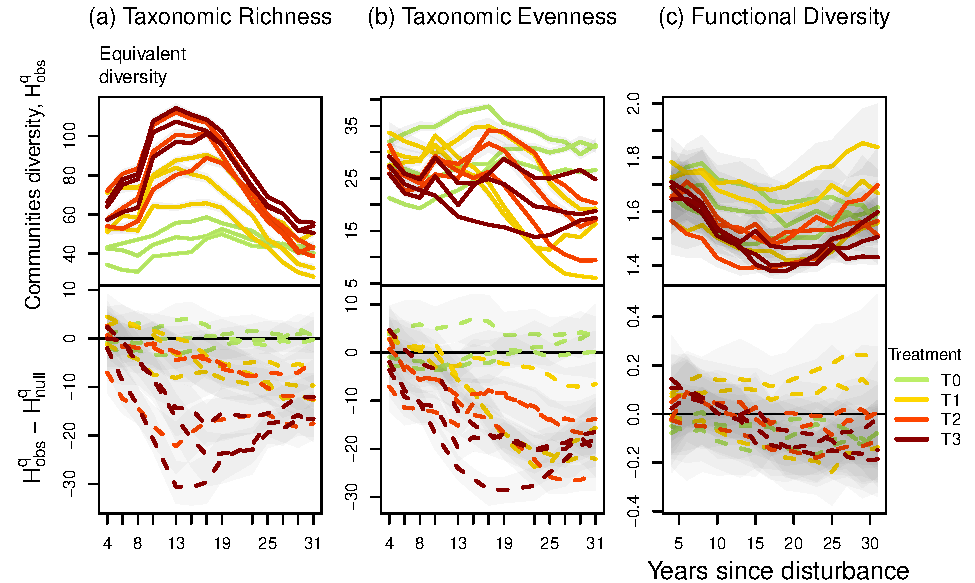
\includegraphics{RecruitmentTrajectories_files/figure-latex/DivTraj-1} 

}

\caption{Upper panels, trajectories over 30 years of taxonomic richness \textbf{(a)}, taxonomic evenness \textbf{(b)} and functional diversity \textbf{(c)} of observed 2-years laps recruitment $H_{obs}^q$. Lower panels, diversity differences to null models $H_{obs}^q - H_{null}^q$}\label{fig:DivTraj}
\end{figure*}

\subsection{Functional composition}\label{functional-composition}

In undisturbed plots functional traits values remained stable over the
30 years while it followed hump-shaped trajectories in all disturbed
plots, to the exception of the leaf chlorophyll content. Trajectories of
SLA and bark thickness first increased before decreasing towards initial
values. Conversely, trajectories of leaf thickness, leaf toughness, wood
specific gravity, and maximum height first decreased and then started
returning towards initial values but their recovery remained unachieved
after 30 years (Figure \ref{fig:CWM}).

\begin{figure*}

{\centering 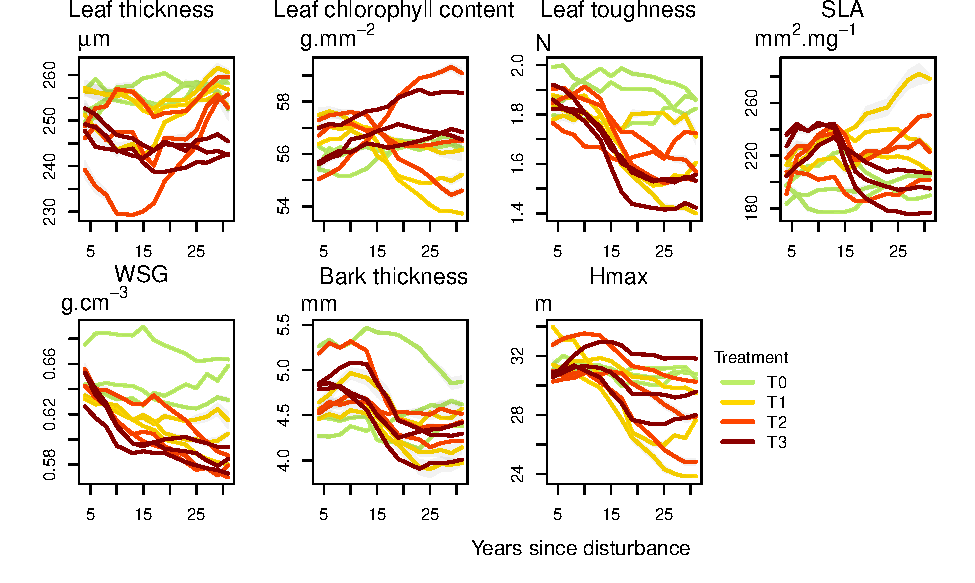
\includegraphics{RecruitmentTrajectories_files/figure-latex/CWM-1} 

}

\caption{Community weighted means (CWM) of the leaf, the two stem and specific maximum height. Shaded areas are the credibility intervals.}\label{fig:CWM}
\end{figure*}

\subsection{Recruitment Turnover}\label{recruitment-turnover}

Over the 30 years in control plots the turnover of recruited species
compared to initial community remained low (Figure \ref{fig:Turnover}).
In disturbed plots the recruited species turnover followed a marked
hump-shaped trajectory, with a maximum reached around 15 years after
disturbance. The maximum turnover was positively correlated to the
disturbance intensity (\(\rho_{spearman}=0.93\)). Thirty years after
disturbance the turnover had returned to low values.

\begin{figure}

{\centering 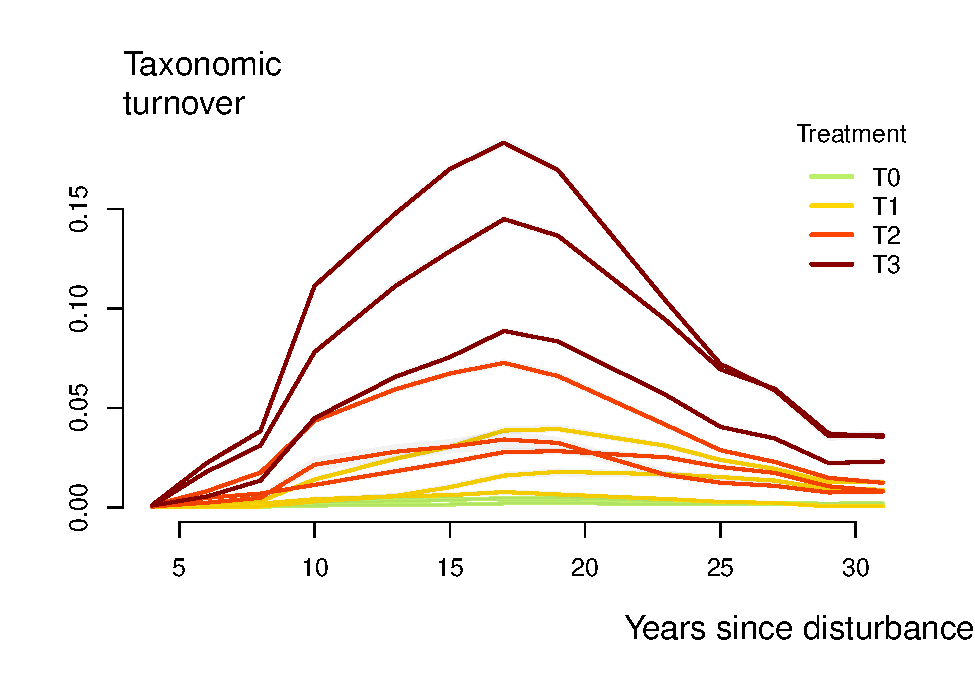
\includegraphics[width=1\linewidth]{RecruitmentTrajectories_files/figure-latex/Turnover-1} 

}

\caption{Trajectories over 30 years of the abundance-based turnover between 2-years laps recruited trees pre-disturbance communities.}\label{fig:Turnover}
\end{figure}

\section{Discussion}\label{discussion}

\subsection{A three-phased deterministic successional
pathway}\label{a-three-phased-deterministic-successional-pathway}

Post-disturbance recruitment trajectories relied on a three-phased
successional pathway defined by the emergence of deterministic
competition processes for light gradually balancing the stochastic
recruitment specific to undisturbed communities.

A first phase (0-8 years), corresponded to the recruitment of
pre-disturbance surviving saplings (DBH \textless{} 10 cm) that
immediately benefited from the increased enlightment and alleviated
competition induced by disturbance \citep{Denslow2000, Herault2010}. The
taxonomic and functional characteristics of recruited trees mirrored the
pre-disturbance communities and recruitment processes matched the null
stochastic recruitment model.

A second phase (8-15 years) was marked by a shift in community
functional composition towards more ``acquisitive'' functional
strategies and the dominance of a restricted set of species. The
recruitment then involved true recruits, \emph{i.e.} trees germinating
from the seeds bank, representing the main part of the whole
post-disturbance recruitment \citep{Lawton1988}. The recruitment was
dominated by short-lived, fast growing hard pioneers displaying
efficient light acquisition \citep{Wright2004, Chave2009b, Herault2011}.
As already demonstrated in temperate forests, the pool of recruited
species was restricted by trait-based deterministic processes favoring
species with efficient light acquisition (high SLA and leaf chlorophyll
content) and inexpensive, short-lived tissues (low leaf thickness and
toughness, small Hmax and low wood specific gravity and bark
thickness)\citep{Chave2004, Kunstler2016}. This emergence of trait-based
deterministic processes balanced the stochastic recruitment observed in
the first place, and the relative importance of both processes was
determined by the disturbance intensity. After low intensity disturbance
(T1 plots) recruited species still mirrored pre-disturbance taxonomic
composition, but included more long-lived pioneers and light-demanding
species \citep{Bongers2009}. For intense disturbance in contrast (T2 and
T3 plots), the composition of recruited trees rapidly differed from
pre-disturbance community and with the high dominance of hard pioneers,
such as \emph{Cecropia spp.} or \emph{Vismia spp.}, likely entailing
significant changes in communities functioning \citep{Diaz2005}.

A third recruitment phase (15-30 years) corresponded to the recovery of
pre-disturbance taxonomic and functional characteristics. Although the
recruits remained mainly light-demanding species their functional
diversity increased and they increasingly resembled the pre-disturbance
taxonomic composition. The deterministic recruitment processes then
gradually left room to stochastic recruitment processes specific to
undisturbed forest \citep{Lawton1988, Chave2004}.

\subsection{The achievement of communities
recovery}\label{the-achievement-of-communities-recovery}

After disturbance the stochastic recruitment specific to undisturbed
communities was progressively restored and drove community taxonomic and
functional recovery. This confirmed previous results from the Paracou
experiment, conducted 10 years \citep{Molino2001} and 20 years
\citep{Baraloto2012a} after disturbance, where the early signs of the
resilience of pre-disturbance taxonomic and functional composition
recovery had been detected.

Recruitment taxonomic richness and evenness recovered pre-disturbance
values and the taxonomic composition converged towards the
pre-disturbance community, thus maintaining the initial differences
among communities for all disturbance intensity. Community taxonomic
convergence to the local pre-disturbance recruitment composition
revealed the scarce recruitment of species that did not belong to
pre-disturbance community, due to the commonness of dispersal limitation
among tropical tree species \citep{Svenning2005}.

Functional composition and diversity trajectories converged similarly in
the functional space towards the recovery of pre-disturbance values,
suggesting a common and resilient functioning despite communities'
taxonomic divergence \citep{Fukami2005}.

Trait-based enhancement processes made deterministic the community
functional response to disturbance but dispersal limitation and
steady-state stochastic recruitment made community taxonomic response
historically contingent. Although resilient, the functional and
taxonomic composition of recruited trees remained altered 30 years after
disturbance by the dominance of light-demanding species. This long-term
impact specifically raises questions for the management of exploited
forests, as most valuable species are late-successional and would thus
require cutting cycles of more than 30 years \citep{Putz2012}.

\section{Conclusion}\label{conclusion}

The post-disturbance recruitment trajectories highlighted a three-phased
deterministic successional pathway shaped by the emergence of niche
processes enhancing light-acquisitive species and balancing the
stochastic recruitment of undisturbed communities. The successional
pathway first corresponded to the enhanced growth of pre-disturbance
surviving saplings mirroring the taxonomic and functional
characteristics of pre-disturbance communities. Second, recruitment
trajectories were shaped by true recruits from the seeds bank selected
through the emergence of competitive exclusion for light fostering
pioneer species. Above a disturbance intensity threshold the second
recruitment phase was dominated by short-lived hard pioneers that
drastically changed community composition, diversity and likely
functioning. A third phase eventually corresponded to the return towards
pre-disturbance recruitment composition and taxonomic and functional
diversity, through the recovery of stochastic recruitment processes
specific to undisturbed communities. Besides, repeated disturbance might
have increasingly strong impacts, as community recovery involved the
seeds bank and probably altered the composition and diversity of the
seeds stock \citep{Norden2009}.

\section{Acknowledgement}\label{acknowledgement}

We are in debt with all technicians and colleagues who helped setting up
the plots and collecting data over years. Without their precious work,
this study would have not been possible and they may be warmly thanked
here.

\section{Data availability}\label{data-availability}

This article is based upon the dataset of the Paracou station, which is
part of the Guyafor permanent plot network in French Guiana
(Cirad-CNRS-ONF). The dataset is available upon request to the
scientific director (https://paracou.cirad. fr).

\begin{center}\rule{0.5\linewidth}{\linethickness}\end{center}

%----------------------------------------------------------------------------------------
%	REFERENCE LIST
%----------------------------------------------------------------------------------------

\bibliographystyle{mee}
\makeatletter
% The filename has .bib extension the must be eliminated
\filename@parse{references.bib}
% parse stores the file name in base. Extension starts at the first dot, so don't use dots in file names.
\bibliography{\filename@base}
\makeatother


%----------------------------------------------------------------------------------------

\end{document}
